\input{./UCLHeader.tex}
%New commands
%Maths
\newcommand{\beq}{\begin{equation}}
\newcommand{\eeq}{\end{equation}}
\newcommand{\bea}{\begin{align}}
\newcommand{\eea}{\end{align}}
\newcommand{\p}{\partial}
\newcommand{\trace}[1]{\mathrm{Tr}\left[#1 \right]}
\newcommand{\ptrace}[2]{\mathrm{Tr}_{#1} \left[ #2 \right]}
\newcommand{\bpmat}{\begin{pmatrix}}
\newcommand{\epmat}{\end{pmatrix}}
\newcommand{\vv}[1]{\vec{#1}}
\newcommand{\mat}[1]{\uuline{#1}}
\newcommand{\norm}[1]{\| #1 \|}
\newcommand{\op}[1]{\mathbb{#1}}
\newcommand{\vhat}[1]{\hat{\vv{#1}}}


%Renewed commands, in order for them to take arguments with automatically adjusted brackets 
\renewcommand{\dim}[1]{\mathrm{dim}\left( #1\right)}
\renewcommand{\det}[1]{\mathrm{det} \left( #1 \right)}
\renewcommand{\exp}[1] {\mathrm{exp} \left[ #1 \right]}


%\mathbb Letters
\newcommand{\identity}{\mathbb{I}}
\newcommand{\inreal}{\mathbb{R}}
\newcommand{\incomplex}{\mathbb{C}}

%Redefine Braket
\renewcommand{\braket}[1]{\left\langle #1 \right\rangle}

%Integration
\newcommand{\intd} {\mathrm{d}}

%Operators
\newcommand{\phihat}{\hat{\phi}}
\newcommand{\xhat}{\hat{x}}
\newcommand{\phat}{\hat{p}}
\newcommand{\Dhat}{\hat{D}}
\newcommand{\Hhat}{\hat{H}}
\newcommand{\ahat}{\hat{a}}
\newcommand{\bhat}{\hat{b}}
\newcommand{\chat}{\hat{c}}
\newcommand{\Phihat}{\hat{\Phi}}

%Channels
\newcommand{\channel}[3]{\mathcal{#1}^{#2 \rightarrow #3}}


%Caligraphy letters
\newcommand{\cl}[1]{\mathcal{#1}}
\newcommand{\Hilbert}{\mathcal{H}}
\newcommand{\calN}{\mathcal{N}}
\newcommand{\Lag}{\mathcal{L}}
\newcommand{\calD}{\mathcal{D}}


%Pauli
\newcommand{\Xhat}{\hat{X}}
\newcommand{\Yhat}{\hat{Y}}
\newcommand{\Zhat}{\hat{Z}}
\newcommand{\PauliX}{\bpmat 0 & 1 \\ 1 & 0 \epmat}
\newcommand{\PauliZ} {\bpmat 1 & 0 \\ 0 & -1\epmat}



%Gell-Mann matrices
\newcommand{\GMone} {\bpmat 0 & 1 & 0 \\ 1 & 0 & 0 \\ 0 & 0 & 0 \epmat }
\newcommand{\GMsix}{\bpmat 0 & 0 & 0 \\ 0 & 0 & 1\\ 0 & 1 & 0\epmat}

%Density matrices
\newcommand{\rhotwo}{\bpmat 1 & e^{-it} \\ e^{it} & 1 \epmat}
\newcommand{\rhothree} {\bpmat 1 & e^{it} & e^{2it} \\
e^{-it} & 1 & e^{it} \\
e^{-2it} & e^{-it} & 1 \epmat}



%Misc
\def\dbar{{\mathchar'26\mkern-12mu d}} %a $d$ with a bar through its stem


\newcommand{\eq}[1]{$#1$}

%Undertilded quantities
\newcommand{\tildeq}{\underset{^\sim}q}
\newcommand{\tildep}{\underset{^\sim}p}

%Curly letters
\newcommand{\calE}{\mathcal{E}}

\newcommand{\Nhat}{\hat{N}}

%Wave vector shortening
\newcommand{\kvec}{\vv{k}}

%Change braket size in ket and bra commands
\renewcommand{\ket}[1]{\left| #1 \right\rangle}
\renewcommand{\bra}[1] {\left\langle #1 \right|}












\begin{document}
\title{Superconductivity Long Notes}
\author{Sofia Qvarfort}
\maketitle

\section{Superconductivity}
\subsection{Weakly interacting dilute Bose gas}
\begin{description}
\item[Full Hamiltonian] is given by 
\beq
H = \sum^N_{i = 1} \left[- \frac{\hbar \nabla^2_i}{2m} + V(r_i)\right] + \sum_{i < j} U\delta (r_i - r_j) 
\eeq

\item[Variational Principle] is the way of finding the minimum energy. We start with a guess for a ground state, then work out the energy. From there, we look at which parameters go into the wavefunction, the minimise the energy from there. 

In the context of superconductivity, the variational principle can be used to find the ground state by minimising the free energy $F$. 

\item[Free energy] is given by
\beq
F = N \int  \intd^3 r \left[ \frac{\hbar^2 }{2m } |\nabla_\chi|^2 + \left( V(r) - \mu \right) |\chi|^2 + \frac{UN(N-1)}{2} |\chi|^4 \right]
\eeq

\end{description}
\section{Classical Josephson Junctions}
\begin{description}
\item[Critical Temperature] called $T_C$, the temperature below which resistivity goes to zero. 

\item[Element with highest $T_C$] is niobium at $9$K. 

\item[Compound with highest $T_C$] is Mercury-Thallium-Barium-Copper-Oxide with 138 K. 

\item[Cooper pairs] are pairs of electrons which form through a mutually attractive pairing interaction. This arises through electron-phonon interactions. 

\item[Spin of electron in a Cooper pair] are always opposing because of the Pauli exclusion principle. 

\item[Meissner Effect] describes the expulsion of magnetic fields from a superconductor. The screening happens through currents appearing in the superconductor, which counter the magnetic field. The superconductor is therefore a perfect diamagnet. 

\item[Magnetic susceptibility] for a superconductor where we observe the Meissner effect is equal to 
\beq
\frac{dM}{dH} = -1
\eeq
Here, $M$ is the magnetisation of the material, which is the magnetic dipole moment per unit volume, and $H$ is the magnetic field strength. 

\item[Penetration depth] is the characteristic length scale for which the magnetic field dies down in the superconductor. The magnetic field decreases exponentially. 

\item[Destruction of superconductivity] occurs at some critical field strength $H_C$, where the material will become resistive and allow magnetic fields into its interior. 

\item[Critical current] called $J_C$ exists, above which the material becomes resistive. 

\item[Conditions for superconductivity] All quantities must be below $T_C$, $H_C$ and $J_C$ for superconductivity to occur. 

\item[Distance between Cooper pairs] can be macroscopic. Therefore, many other Cooper pairs can reside within the same area. This causes the electrons to move coherently. 

\item[Wavefunction] for electrons in a superconductor can be written down with a single pair wavefunction
\beq
\tilde{\psi}(+vv{r}) = |\psi(\vv{r})|e^{i \theta (\vv{r})}
\eeq

\item[Origin of zero resistance] is the fact that macroscopic electron pairs behave coherently. If an electron pair scatters off a phonon, the other Cooper pairs will move to compensate the phase difference. 

\item8Superconducting coherence length] usually written $\chi$, and is derived from the Cooper pair length. It can also be thought of as the characteristic exponent of the variations of density of the superconducting component. In BCS theory, it is given by 

\beq
\chi = \frac{\hbar v_f}{\pi \Delta}
\eeq
where $v_f$ is the Fermi velocity and $\Delta$ is the superconducting energy gap. 

Also, it can be found that 
\beq
\xi \propto \frac{1}{T_C}
\eeq
which is bad news for high temperature superconductors. 

One consequence of the coherence of the electrons is that we can find many quantum phenomena in superconductors, such as emulating the Young's slit experiment. 

\item[Defects] in a superconductor do not influence the behaviour as long a they are smaller than the superconducting coherence length $\xi$. 

\item[Number density of superconducting electrons] is given by the probability of detecting an electron at position $\vv{r}$, so that 
\beq
n_s( \vv{r}) = |\psi(\vv{r})|^2
\eeq

\item[Superconducting order parameter] is the absolute amplitude of the wavefucntion, $|\psi|$. It provides a measure of `how strong' the superconductivity in a sample is. It is related to the density of Cooper pairs. 

\item[Magnetic flux through superconducting loop] is \emph{quantised}. This follows from the phase coherence. Boundary conditions stipulate that the phase must differ by $2\pi$ if you go around the loop once. 

\item[Flux quantum] the minimal flux that is allowed through a superconducting loop, given by 
\beq
\phi_0 = \frac{h}{2e}
\eeq



\end{description}

\subsubsection{Type I and type II superconductors}
\begin{description}
\item[Type I superconductor] reaches its normal state immediately after the external magnetic field $H$ reaches $H_C$. 

\item[Type II superconductor] reaches its normal state gradually and not abruptly once the critical field $H_C$ has been applied. For fields below $H_C$, the magnetic flux creates discrete Abrikosov current vortices that shield the incoming field. Each vortex carries on thread of magnetic field with one flux quantum. 

As the external magnetic field increases, more and more vortices appear. Finally, the whole sample is filled with vortices, and it becomes normal (resistive) again. 

\item[Abrikosov vortex] appears in a Type II superconductor in an external field which is lower than $H_C$. A vortex can also be called a fluxon. The normal region in the vortex through which magnetic field can penetrate. 

Question: Is this just the `void' that appears in a superfluid? 

The circulating part is the current, which screens exactly one $\phi_0$. 

\item[Size of a vortex] the radius is of the scale of the penetration depth $\lambda$. We know that magnetic fields are screened on a length scale of $\lambda$, and therefore we can think of the vortex as extending over this length and shielding one flux quantum along it. 

The normal core of the vortex (where we have no shielding current) is of size $\xi$. This is because coherence can be maintained over this length scale. 

Question: I don't think I have a good, intuitive grasp on this. 

Attempt at answer: 

\item[Characterisation of Type I or Type II] we note that: \\ 
- Type I: $\frac{\lambda}{\xi} < \frac{1}{\sqrt{2}}$ \\
- Type II: all other cases. 

\end{description}
\subsubsection{The Energy Gap and Quasi Particles}
\begin{description}

\item[Energy required to break Cooper pair] is $2\Delta$. 

\item[Temperature dependence] we find that\\
- At $T = 0$ there are no phonons, just Cooper pairs \\
- At $0 < T< T_C$ there is a small but finite phonon density which can break pairs.  \\
- At $T = T_C$, all Cooper pairs have been broken \\

Note that we find that the density of Cooper pairs obeys
\beq
n \sim \frac{1}{T}
\eeq

\item[Breaking a Cooper pair] creates two quasi-particles, not electrons. A quasi-particle in a superconductor is a superposition of an electron-like particle and a hole-like particle. Resulting quasi-electrons and quasi-holes have energy $\Delta $ more than the rest of the Cooper pairs. There is an energy difference of $2\Delta$ between the `electron' and the `hole'. 

The states which above $T_C$ were within the energy gap get `pushed out' to the edge of the gap. The result is a large peak in the quasi-electron and quasi-hole densities of states at the gap edge.  

\item[Density of quasi-particle states] is given by
\beq
N_{qp} (E) = N_0 \mbox{Re} \left( \frac{E}{\sqrt{E^2 - \Delta^2}}\right)
\eeq
where $N_0$ is the single-spin density of states in the normal state. 

Question: Derivation?

\item[Electric field] causes the quasi-particles, as they move through it, they cause dissipation. At DC, the quasiparticle current is always shorted by the non-dissipative Cooper pair current. 

Question: I don't understand the last sentence. 

\item[Two-fluid model] a model for describing the conductivity of a superconductor at finite temperatures. Here, current flow is modelled as carried by $n_s$ paired electrons and $n_n$ quasi-particles. For this model, we neglect pair-breaking, by assuming that 
\beq
\frac{\omega}{2\pi} < \frac{2\Delta}{h}
\eeq

The two-fluid model attempts to explain superconductivity in e.g. liquid He below the lambda point. The components are a normal fluid and a superfluid component. Together their sum makes up the total density. 


\item[Charge conservation] the number of electrons in the normal state (above $T_C$) is given by 
\beq
n = n_s + n_n
\eeq


\item[Electric field response] the Cooper pairs move with velocity $\vv{v}_s$ and do not experience momentum-scattering collisions. The quasi-particles move with velocity $\vv{v}_n$ and experience momentum-scattering collisions at an average rate $\tau$. 

We find
\beq
2m \frac{d \vv{v}_s}{dt} = - 2e \vv{E}
\eeq
\beq
m\frac{d \vv{v}_n}{dt} = - e \vv{E} - m \frac{\vv{v}_n}{\tau}
\eeq
where $m$ is the mass of charge carriers, equal for paired electrons and quasiparticles. Note that the second term of the second equations implies a drag force. 

Question: Where does the factor of 2 in the first equation come from? 

\item[Current density ] for Cooper pairs and quasi-particles given by 

\beq
\vv{J} = - n_s e\vv{v}_s - n_n e \vv{v}_n
\eeq

\item[Conductivity] we assume that the electric field is harmonic and of the form 
\beq
\vv{E} = \vv{E}_0 e^{i \omega t}
\eeq
then we define real and imaginary conductivities from the current, 
\beq
\vv{J} = ( \sigma_1 - i \sigma_2 ) \vv{E}
\eeq
to obtain
\beq
\sigma_1 = \frac{n_n e^2 \tau}{(1 + \omega^2 \tau^2) m}
\eeq
\beq
\sigma_2 = \frac{n_s e^2 }{m \omega} + \frac{n_n e^2 (\omega \tau)^2}{(1 + \omega^2 \tau^2 ) m \omega }
\eeq

$\sigma_1$ describes the dissipative loss when a superconductor is excited by an electric field at frequency  $\omega$. It limits the Q factor of superconducting microwave resonators in Josephson qubit devices. 



Question: This needs a derivation, will get to it...



\end{description}

\subsubsection{Low $T_C$ and high $T_C$ superconductors}
\begin{description}
\item[Low $T_C$ superconductor] are metallic elemental and alloy superconductors. 

\item[High $T_C$ superconductors]  are usually made of compounds. 

\item[Differences between low $T_C$s and high $T_C$s] are the following:
\begin{itemize}
\item Pairing mechanism in low $T_C$ given by the BCS virtual phonon interaction. In high $T_C$, it is unknown. 
\item Properties of $T_C$s are anisotropic. 
\item For copper compounds, electrons that move in parallel to the cuprate planes obtain a band gap that displays four-fold symmetry. Nodes appear in the value of the gap every 90 degrees. This energy gap depends on the momentum of the paired electrons. 
\item For high $T_C$s, the properties can be tuned by doping, usually by increasing the number of oxygen atoms. 
\item The coherence length is small in high $T_C$s. It is limited by the motion of fluxons in the Lorentz force. 
\end{itemize}

Question: I presume then that the properties of low $T_C$s are generally isotropic? 


\end{description}
\subsection{Classical Properties of Josephson Junctions}
\subsubsection{Basics}
\begin{description}
\item[Josephson junction] consists of two superconducting thin films with a barrier between them. The wavefunctions $\psi_1$ and $\psi_2$ in respective section are weakly coupled. 

\item[SIS Josephson junction] is made of two superconducting thin films and an insulator. 

\item[SNS Josephson function] is made of two superconducting thin films separated by a normal metal. 


\item[Quantum behaviour] of the Josephson junction comes from the interference between the two wavefunctions
\beq
\phi = \phi_1 - \phi_2
\eeq

\item[Josephson equations] are
\beq
I_S = I_C \sin{\phi}
\eeq
\beq
V = \frac{\hbar}{2 e} \frac{\p \phi}{\p t}
\eeq
Note that $I_S$ is a supercurrent that flows through the device. This is a macroscopic quantum phenomenon. 


\item[Static solution] can be obtained when
\beq
I_S < I_C
\eeq
as we can then obtain the phase $\phi$ from the equations above. This means that $\phi$ is static, and the voltage $V$ is zero. 

\item[Unstable solution] if
\beq
I_S > I_C
\eeq
we can obtain no stable value for $\phi$ and thus $V$ is finite across the junction. 

\end{description}
\subsubsection{Resistively-Shunted junction model}

\begin{description}
\item[Contributions to the current across a Josephson junction] given by
\begin{itemize}
\item The Josephson supercurrent $I_S$ 
\item A current from the capacitance induced over a Josephson function 
\beq
I = C\frac{dV}{dt}
\eeq
\item A current formed from tunneling of quasi-particles across the junction. 
\end{itemize}

\item[Non-linear differential current equation] one can combine the above contributions to the current to write
\beq
I = I_C \sin{\phi} + \frac{\hbar} {2eR} \frac{\p \phi}{\p t} + \frac{\hbar C}{2 e} \frac{\p^2 \phi}{\p t^2}
\eeq
This can be solved numerically, but see washboard model for physical intuition. 

\end{description}
\subsubsection{Washboard model}
\begin{description}
\item[Washboard model] provides intuition about the non-linear behaviour of the supercurrent $I$ across the Josephson junction. 

\item[Washboard potential] from comparison with non-linear equation above, given by 
\beq
U(\phi) = - \frac{\hbar}{2e} \left( I_C \cos{\phi} + I \phi \right)
\eeq


\item[Rolling ball analogy] the behaviour of a ball of mass $m$ that rolls along a periodic washboard describes the dynamics pretty well. Properties:
\begin{itemize}
\item Horizontal position of ball = phase difference $\phi$
\item Viscous drag force on ball = dissipative current
\beq
F_{drag} = \frac{1}{R} \left( \frac{\hbar}{2e} \right)^2 \frac{\p \phi}{\p t}
\eeq
\item Mass of ball = proportional to capacitance $C$ of junction
\beq
m = \left( \frac{\hbar}{2e} \right)^2 C
\eeq
\item Velocity of ball = voltage across the junction
\end{itemize}

\item[Natural oscillation frequency] where the ball wiggles around in its local minima is given by 
\beq
\omega_A = \omega_P \left( 1 - \left( \frac{I}{I_C} \right)^2 \right)^{1/4}
\eeq
where $\omega_P$ is the plasma frequency. 

\item[Josephson plasma frequency] is the oscillation frequency when the net current is zero, given by 
\beq
\omega_P = \left( \frac{2 e I_C}{\hbar C} \right)^{1/2}
\eeq

Question: What here is actually oscillating? 

Attempt at answer: We said that the horizontal position of the ball is the phase difference. Therefore, it is probably the phase different that oscillates. 
\end{description}
\subsubsection{Washboard model $T= 0$}
Here we assume negligible damping. 

\begin{description}
\item[At $I = 0$] the ball is trapped in one of the minima, so
\beq
\frac{d\phi}{dt} = 0 
\eeq
which implies that $V = 0$. 

\item[Josephson energy] given by
\beq
E_J = \frac{\hbar I_C}{2e}
\eeq
where $2 E_J$ is the height of the potential barrier at $I = 0$. 

\item[Non-zero $I$] means that we have a  potential step

\beq
\Delta U\simeq 2E_J \left( 1 - \frac{I}{I_C} \right)^{3/2}
\eeq
which means that the ball can escape. With no damping, the ball keeps rolling down the washboard. 

\item[At critical current $I_C$] we see that $\Delta U = 0$. This means that 
\beq
\frac{d \phi}{dt} \neq 0
\eeq
 throughout which implies finite $V$. 
 
 \item[Below the critical current $I_C$] the ball can keep rolling. It keeps rolling until the current is reduced to zero. 
 
 \item[Hysteretic] since the ball keeps moving until $I = 0$ if we are decreasing the current, but doesn't start rolling until $I = I_C$ if increasing the current, we conclude that the system displays hysterecis. 
 
 \end{description}
 
\subsubsection{Washboard model: $T>0$ with negligible damping}
\begin{description}

\item[Brownian motion] the ball will undergo Brownian motion when it sits in the minima. The amplitude of the random walk increases with increasing $T$. This causes the ball to escape even at $I < I_C$.  The average time it takes to escape is
\beq
\tau_{TA}^{-1} = \frac{\omega_A}{2\pi} e^{- \Delta U/k_B T}  
\eeq

\item[Average number of escape attempts] per second given by $\omega_A /1 \pi$. 

\item[Switching current] written $I_{sw}$ is the value of the current at which the ball escapes by thermal fluctuation. The same $I_{sw}$ will not be found by repeating the measurement. 

\end{description}
\subsubsection{Washboard model: $T>0$ with damping}
\begin{description}
\item[Behaviour] now the ball experiences a drag force and will stop after travelling over a set number of minima. 

\item[Quality factor] called $Q$ denotes the damping in the system. It is given by 
\beq
Q = \omega_P RC
\eeq

\item[McCumber parameter] another way to measure the quality of a Josephson junction. Written
\beq
\beta_C = Q^2
\eeq


\item[Hystereic junctions] are junctions with 
\beq
Q>3
\eeq
These junctions are also known as underdamped. 

\item[Non-hysteretic junctions] have smaller $Q$ and are called overdamped. 



\end{description}

\subsection{Radio-Frequency effects in Josephson Junctions}
\begin{description}
\item[External DC voltage] which is constant means we can solve for the phase using one of the Josephson equations, 
\beq
\phi(t) = \frac{2e}{\hbar} Vt + \phi_0
\eeq
Substitute this into the first equation to get the current:
\beq
I_S = I_C \sin{\left( \frac{2e}{\hbar} Vt + \phi_0 \right)}
\eeq

\item[Supercurrent oscillation frequency] for an external voltage given by
\beq
f_J = \frac{1}{2\pi} \frac{2e}{\hbar} V
\eeq

\item[Josephson effect] is what we call the fact that the supercurrent flows across the Josephson junction. 



\end{description}
\subsubsection{Shapiro steps}
\begin{description}
\item[External RF voltage] if the voltage is no longer constant but time-dependent, $Vl(t)$, we integrate the Josephson equation to find
\begin{align}
I_S(t) &= I_C \sin{\left( \int^t_0 \frac{2e}{\hbar} v(t') \intd t' + \phi_0 \right) } \\
&= I_C \sin{\left( \frac{2eV}{\hbar} t + \frac{2eV_s}{\hbar \omega_s} \sin{\left( \omega_s t\right)} + \phi_0 \right)}
\end{align}
where $\omega_s$ is the frequency of the voltage source. 

Also note that 
\beq
v(t) = V + V_s\cos{\omega_s t}
\eeq

Question: What is the $V_s$ voltage?  

Attempt at answer: This is maximum amplitude of the oscillating voltage source. 

\item[Bessel function] are canonical solutions $y(x)$ of Bessel's differential equation:
\beq
x^2 \frac{d^2 y}{dx^2} + x \frac{dy}{dx} + (x^2 - \alpha^2 ) y = 0
\eeq
for a complex number $\alpha$. 

\item[Occurrence of Shapiro steps] current equation contains a Bessel function can be expanded to give
\beq
I_S(t) = I_C \sum_{n = - \infty}^\infty (-1)^n J_n \left( \frac{2eV_s}{\hbar \omega_s} \right) \sin{\left( (\omega_J - n \omega_s ) t + \phi_0 \right)}
\eeq

An interesting solution occurs when the source frequency is a multiple of the Josephson frequency $\omega_J = n \omega_s$. Then we see the 

\item[Shapiro steps for voltage standard] by connecting $N$ Josephson junctions together, we get very accurate Shapiro steps. They are given by 
\beq
V  = N \frac{\pi \hbar }{2} f_J
\eeq
The voltage is thus entirely determined by fundamental constants and the $f_J$, which can be precisely measured. 

\end{description}

\subsection{Josephson Junctions in a Magnetic Field}
\begin{description}
\item[Effect of $B$ field on superconducting ring ] is that we induce a phase change. Can show that 
\beq
\Delta \phi = \frac{2e}{\hbar} \int^B_A \vv{A} \cdot \intd \vv{l}
\eeq
That is, the field must be quantised. 

\item[Effect of $B$ field on Josephson junction] the total phase difference does not both depend on the difference between the two materials and the phase induced by the external magnetic field. We find
\beq
\phi = \phi_1 - \phi_2 + \frac{2e}{\hbar} \int \vv{A} \cdot \intd \vv{l}
\eeq
Note that we integrate from the interior of one of the superconducting films to the interior of the other one. 

The effect is that we can very accurately control the junction by applying an external magnetic field. 

\item[Spatially varying magnetic field] creates changes in the phase $\phi(x)$ that are in turn position dependent. We must rewrite
\beq
j_S(x) = j_c \sin{\phi (x)}
\eeq
where $j_s(x)$ is the supercurent density per unit width in the $x$ direction and $j_c$ is the  critical current density. 

\item[Calculating the total phase] we can show that (by integrating over an area inside the superconductor) that
\beq
\phi(x) - \phi(0) = 2\pi \frac{\Phi(x)}{\Phi_0}
\eeq
where
\beq
\Phi(x) = \frac{\Phi x}{w}
\eeq
and where $w$ is the width of the junction (I think). 
Question: Should $\Phi$ actually be $\Phi_0$? 
Question: I do not know what the $\Phi(x)$ term is, unless it is just a dummy variable that we have treated. 

\item[Total current under external field] is given by integrating the previous equation, 
\begin{align}
I_S &= \int^{w/2}_{- w/2} \intd x j_c \sin{\left( \phi(0) + 2 \pi \frac{\Phi(x)}{\Phi_0} \right)} \\
&= \frac{j_c w \Phi_0}{\pi \Phi} \sin{\left( \phi(0)\right)} \sin{\left( \frac{\pi \Phi}{\Phi_0} \right) }
\end{align}

\item[Maximum superurrent] that can flow through the function occurs when
\beq
\phi(0) 0 \pm \frac{\pi}{2}
\eeq
for which we obtain
\beq
I_C( \Phi) = I_c(0) \left| \frac{\sin{\left( \frac{\pi \Phi}{\Phi_0} \right) }}{\left( \frac{\pi \Phi}{\Phi_0} \right) } \right|
\eeq



\item[Critical current in zero magnetic field] is given by 
\beq
I_C(0) = j_c w
\eeq
where again $j_c$ is the critical current density and $w$ is the width of the side of the junction that runs parallel to the barrier. 

\item[Flux required to suppress critical current] is equal to one flux quantum $\phi_0$. 

Question: Is this really correct? 

Attempt at answer: Before, we said that certain superconducting properties were the same for every superconductor. However, I would have thought that we require more than one flux quantum to cancel the critical current. Although I might misunderstand. I assume that the critical current is what we whip up in order to cancel out the magnetic field. So something is wrong here. 

\end{description}

\section{Fabrication and measurement of Josephson junctions}
\subsection{Fabrication of low $T_C$ Josephson junctions}
\begin{description}
\item[Double-angle shadow evaporation] of aluminium films with aluminium oxide barriers exploits that evaporated Al atoms will travel in a straight line from the source to the substrate. Some of the substrate is protected by a mask through which the deposition is made. The mask is a suspended bi-layer resist mask fabricated using either photolithography or EBL. 

The procedure is as follows:
\begin{itemize}
\item Apply the mask
\item Evaporate the first Al layer onto the substrate
\item Allow oxygen into chamber of oxidise the Al
\item Rotate sample
\item Evaporate other side of Al
\end{itemize}


\item[`Whole wafer' Niobium Trilayer Junctions] Evaporating Nb is impossible due to its high melting point. Therefore, we grow Nb by sputter deposition. Sputter deposition is done by accelerating argon ions towards a Nb target so that Nb atoms are emitted and form a film on a nearby substrate. Nb atoms will not travel in straight line because there is Argon in the chamber. Then, the AlO layer is grown on it without breaking vacuum. 


\end{description}


\subsection{Measurement of Josephson junctions}
\begin{description}
\item[Typical measurement] consists of controlling an external magnetic field and current while measuring the ingoing and outgoing current. It has to be done in cryogenic temperatures for the junction to remain superconducting. 

\item[Shielding] the junctions must be shielded from stray electromagnetic fields (earth of mains) and from RF interference. 

\item[DC wiring to junction] is done with twisted pairs (to cancel picked-up RF on both lines) or with mini coaxial cables. A coaxial cable has an inner conductor surrounded by a tubular insulating layer, surrounded by a tubular conducting shield. 

\item[Minimising RF coupling] apart from coaxial cables and twisted pairs, we also add low temperature powder filters. 

\item[Current bias] the junctions are usually current biased because they have very low resistance. 

\item[Four terminal configuration] is used so that the potential difference across the wiring of the sample and any contact resistance is not measured. 

\item[Cryo-CMOS] amplifiers don't work at the temperatures where Josephson junctions operate. Therefore, we need to use special heavily doped silicon amplifiers or SQUIDs to amplify the signal. 

\item[Magnetic shielding] the full sample can be shielded by a superconducting shield or a material with a high permeability (mu metal) which collects the magnetic field lines inside itself. 

\end{description}

\section{Ed Roman's Lecture - SQUIDS}
\subsection{Introduction}
\begin{description}
\item[SQUIDS] are ultrasensitive magnetic flux sensors. They can be thought of as flux-to-voltage transducers. 

\item[Applications] include measuring:

\begin{itemize}
\item very small magnetic signals
\item measure/amplify small currents or voltages
\item measure any quantity that can be related to magnetic flux
\end{itemize}

\item[Flux quantisation] occurs for a superconducting ring. Only an integer $n$ number of flux quanta $\phi_0$ are allowed into the ring .This follows from the fact that the phase $\theta$ of the wavefunction must be \emph{unique}. It therefore changes by $2\pi$ (goes to its original value) after one turn around the ring. Can show
\beq
\Delta \theta = \frac{2 e}{\hbar} \int_S \vv{B} \cdot \intd \vv{S} = \frac{2e}{\hbar} \phi
\eeq
where $\phi$ is the total magnetic flux. 

\item[Flux quantum] defined by 
\beq
\phi_0 = \frac{h}{2e}
\eeq

\item[Commercial Josephson junctions ] are fabricated using conventional photolithography in a cleanroom with the structure defined by etching. We want junctions to have
\beq
\beta_C < 1
\eeq
to avoid hysteresis. This is done by first fabricating them with $\beta_c >1 $ and then adding a metal resistor in parallel with the junction. This gives non-hyesteretic behaviour. 

\end{description}
\subsection{DC SQUIDS}
\begin{description}

\begin{figure}[h]
  \caption{DC SQUID.}
  \centering
    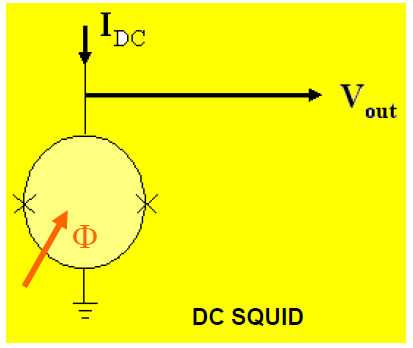
\includegraphics[width=0.5\textwidth]{./SC_figures/DC_SQUID.PNG}
\end{figure}

\item[DC SQUID] consists of two Josephson junctions that are connected by a superconducting loop. We interface with the SQUID by inputting a current into the loop or applying a magnetic field perpendicular to the loop crosssection. 

\item[Josephson junction analogue] One can think of a Josephson junction as a non-linear inductance which accumulates magnetic field energy when a current passes through it. However, the accumulated energy is not expressed in the magnetic field. It is rather thought of as the Josephson energy. 


\item[Measurement of DC SQUID] is done by applying an external current $I_b$ into the SQUID (see figure). This is also called the \emph{measurement current}. We measure the voltage over the entire SQUID by comparing the output voltage $V_{out}$ to ground. 

\item[Measured critical current] is $2I_c$, where $I_c$ is the critical current of one single junction. Since we have two junction, and the electrons have two paths to choose from, we can achieve double the critical current before superconductivity breaks down. 

\item[Circulating supercurrent] will be given by 
\beq
J = \frac{\phi_{ext}}{L}
\eeq
where $L$ is the inductance of the Josephson junction. 

\item[Current in the junctions] is given by 
\beq
I_{net} = \frac{I_b}{2} \pm J
\eeq
depending on which way the magnetic flux comes in. 

\item[$I_c$ flux dependence] is as follows:  as we increase $\phi$, $I_c$ decreases until we hit $\frac{1}{2} \phi_0$. Then it becomes more energetically favourable to change the direction of the supercurrent, after which $I_c$ starts to increase again. 

Note: I recall Ed saying that this was a fairly handwavy argument... 

The reason for the $\frac{1}{2} \phi_0$ increase is because we gain $\frac{1}{2} \phi_0$ from the supercurrent and $\frac{1}{2} \phi_0$ from the measurement current. At all times, the flux in the loop remains quantised. 

\item[Maximum flux sensitivity] is achieved by maximising the largest possible modulation of the SQUID current. Requirements:
\begin{itemize}
\item Loop inductance $L$ \emph{as small as possible}
\item $J$ as large as possible
\item Screening parameter condition
\beq
\beta_L  = 2 \frac{LI_c}{\phi_0} \leq 1
\eeq
\end{itemize}


\item[Screening parameter] written $\beta_L$ is related to the hysteresis of the SQUID. 

Question: I don't yet know in which way. 

\item[Geometric loop inductance] $L$ generally scales with the circumference of the loop. Thus we often strive to increase the effective area of the SQUID. 


\item[Measuring magnetic flux] can be done by fixing the current, usually just above $2I_c$ and measuring the change in voltage $V$. The voltage will oscillate as a function of $\phi$. Note the hyesteretic behaviour in the graph below. 

\begin{figure}[h]
  \caption{Constant current dependence.}
  \centering
    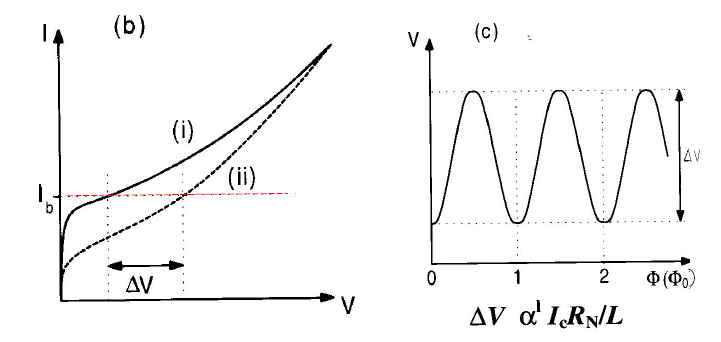
\includegraphics[width=\textwidth]{./SC_figures/Constant_Current_Measurement.PNG}
\end{figure}

The Voltage amplitude $\Delta V$ depends on how we set the external measurement current $I_B$. We want to hit the largest $\Delta V$ so that the oscillations are large. Then we obtain very fine readings for the magnetic flux. 

\item[Relative flux sensor] Because of the periodicity, the squid cannot sense absolute magnetic field, just changes in magnetic field strength. 

\item[Voltage modulation depth] $\Delta V$ is roughly given by 
\beq
\Delta V \sim \frac{I_c R_N}{1 + \beta_L}
\eeq
where $R_N$ is the junction normal resistance. For the ideal $\Delta V$, we require, 
\beq
\beta_L \leq 1
\eeq

\item[Switching voltage] is given by 
\beq
V_{switch} = I_c R_N
\eeq
Its maximum value is $\frac{1}{\Delta}$ where $\Delta$ is the energy gap of the superconductor. 

\item[Small signal mode] is an operational mode of the SQUID where we measure $\phi \ll \phi_0$. It is also known as the \emph{voltage state}. The procedure is as follows:
\begin{itemize}
\item Tune $I_b$ to maximise $\Delta V$
\item Add a fixed $B$ field to sit at a steep part of the curve, e.g. $\frac{\phi_0}{4}$
\item Measure the transfer function $\delta V = V_\phi \delta \phi$ where
\beq
V_\phi = \frac{d V}{d\phi} \bigg|{max} \sim \frac{R_N}{L}
\eeq
\item Obtain change  $\delta \phi$ in external flux
\end{itemize}



Question: What exactly is the switching voltage? 



\item[Noise in voltage state] sets the sensitivity of the SQUID. At most frequencies, the limitation is thermal (Johnson) noise. At lower frequencies, the sensitivity is limited by $1/f$ noise. All frequencies suffer white noise. 

\item[Johnson-Nyquist noise] is the electric noise generated by the thermal movement of electrons inside a conductor. The derivation of this noise is called the fluctuation-dissipation theorem. 

The total amount of thermal noise measured across a resistor depends on the measurement bandwidth $\Delta f$ of the instrument. 

\item[$1/f$ noise] also called pink noise where the frequency spectrum has a power spectral density that is inversely proportional to the frequency of the signal. 

\item[White noise] is a random signal with a constant power spectral density. 

\item[Power spectral density] is the mean square voltage per unit bandwidth. That is
\beq
\frac{V^2}{Hz}
\eeq

\item[Theoretical minimum power spectral density] for a SQUID has through simulations been found to be
\beq
S_V(f) \sim 16 k_B T R_N
\eeq
at the small signal operating point. 

\item[Flux noise] the power spectral density of the equivalent flux noise is given by 
\beq
S_\phi(f) \frac{\sim S_V(f)}{V^2 _\phi} \simeq \frac{16 k_B TL^2}{R_N}
\eeq

\item[Maximising sensitivity of the SQUID] is done by minimising $S_\phi(f)$. This is done by 
\begin{itemize}
\item Low $L$
\item Low $T$
\item High $R_N$
\end{itemize}
Note that the increase in $R_N$ will be compensated by the increase in $V^2_\phi$. 






\end{description}
\end{document}